\documentclass[12pt, a4paper]{article}

% Text languages
\usepackage[english, UKenglish, USenglish, american, british]{babel}

% Accents
%usepackage[latin1]{inputenc}

% Maths
\usepackage{mathtools}
\usepackage{amsmath,amsthm,amssymb}

% Double rows
%\usepackage{multirow}

% Math-mode symbol & verbatim
%\def\W#1#2{$#1{#2}$ &\tt\string#1\string{#2\string}}
%\def\X#1{$#1$ &\tt\string#1}
%\def\Y#1{$\big#1$ &\tt\string#1}
%\def\Z#1{\tt\string#1}

% A non-floating table environment.
%\makeatletter
%\renewenvironment{table}%
%   {\vskip\intextsep\parskip\z@
%    \vbox\bgroup\centering\def\@captype{table}}%
%   {\egroup\vskip\intextsep}
%\makeatother

%\DeclarePairedDelimiter\abs{\lvert}{\rvert}%
%\DeclarePairedDelimiter\norm{\lVert}{\rVert}%

% Swap the definition of \abs* and \norm*, so that \abs
% and \norm resizes the size of the brackets, and the 
% starred version does not.
%\makeatletter
%\let\oldabs\abs
%\def\abs{\@ifstar{\oldabs}{\oldabs*}}
%
%\let\oldnorm\norm
%\def\norm{\@ifstar{\oldnorm}{\oldnorm*}}
%\makeatother

% C++
\usepackage{listings}
\usepackage{xcolor}
\lstset { %
	language = C++,
	backgroundcolor=\color{black!5}, % set backgroundcolor
    basicstyle=\footnotesize,% basic font setting
    tabsize=4, % tab space width
    showstringspaces=false, % don't mark spaces in strings
    %numbers=left, % display line numbers on the left
    commentstyle=\color{green}, % comment color
    keywordstyle=\color{blue}, % keyword color
    stringstyle=\color{red}, % string color
    linewidth=16cm
}

% https://www.overleaf.com/learn/latex/Page_size_and_margins
\usepackage{geometry}
\topmargin = -23pt
\oddsidemargin = 13pt
\headheight = 12pt
\headsep = 25pt
\textheight = 674pt
\textwidth = 426pt
\marginparsep = 10pt
\marginparwidth = 50pt
\footskip = 30pt
\marginparpush = 5pt
\hoffset = 0pt
\voffset = 0pt
\paperwidth = 597pt
\paperheight = 845pt

% Hyperlinks
\usepackage{hyperref}

% Figure
\usepackage{graphicx}
\usepackage{caption}
\usepackage{subcaption}
\usepackage{etoc}
% Example
\newtheorem{exmp}{Example}[section]
% Algorithms
%\usepackage[]{algorithm2e}
%\usepackage{algorithm}% http://ctan.org/pkg/algorithm
%\usepackage{algpseudocode}% http://ctan.org/pkg/algorithmicx
\usepackage{algpseudocode}

\renewcommand{\thefootnote}{\arabic{footnote}} % 1, 2, 3... (la que hay por defecto)

\setcounter{secnumdepth}{5}
\setcounter{tocdepth}{5}

%\titleformat{\paragraph}
%{\normalfont\normalsize\bfseries}{\theparagraph}{1em}{}
%\titlespacing*{\paragraph}
%{0pt}{3.25ex plus 1ex minus .2ex}{1.5ex plus .2ex}

\usepackage{float}
%--------------------------------------------------------------------------
\title{PARALLELISM}
\author{Roger Vilaseca Darné and Xavier Martín Ballesteros\\
  \small UNIVERSITAT POLITÈCNICA DE CATALUNYA\\
}
\date{10th December 2018}

\begin{document}
% Images
\graphicspath{ {./images} }

%\maketitle

\begin{titlepage}
	\centering
%	{\scshape\LARGE UNIVERSITAT POLITÈCNICA DE CATALUNYA \par}
	\vspace{1cm}
	{\scshape\Large UNIVERSITAT POLITECNICA DE CATALUNYA\par}
	\vspace{1.5cm}
	{\huge\bfseries PARALLELISM\par}
	\vspace{2cm}
	{\Large\itshape \textbf{Lab 5: Geometric (data) decomposition:
heat diffusion equation}\par}
	\vfill
	{\Large\itshape Roger Vilaseca Darne and Xavier Martin Ballesteros\break PAR4110\par}
	\vfill
	
\includegraphics[width=0.25\textwidth]{./images/UPC.png}\par\vspace{1cm}
	%supervised by\par
	%Dr.~Mark \textsc{Brown}

	\vfill

% Bottom of the page
	{\large 7th June 2019, Q2}
\end{titlepage}

%\abstract{Esto es una plantilla simple para un articulo en \LaTeX.}

%	*********************** ÍNDEX *********************
\setcounter{secnumdepth}{5}

\newpage
  \tableofcontents
\newpage

% Referència a una equació \ref{eq:area}).
% Referència a una secció \ref{sec:nada}
% Referència a una cita \cite{Cd94}.

\section{Introduction}

\section{Analysis with \textit{Tareador}}

In this section we have used the \textit{Tareador} tool to analyse the possible parallelism strategies that we can use in order to parallelise both Jacobi and Gauss-Seidel solvers. 

We have mainly focused on the data dependences that appear and how will we protect them in our parallel \textit{OpenMP} code. To explore the dependences, we have used a much finer task decomposition: one task for each iteration of the body of the most innerloop.

\subsection{Jacobi Solver}

This solver uses an auxiliar matrix \textbf{utmp} to write the resulting values of the computation in the most innerloop of the body. For each element in the matrix \textbf{u}, it takes the values of the element on its top and bottom and on its left and right, and does some arithmetic operations.

The modified code using the \textit{Tareador} tool is shown below. However, the code can be found in \textit{jacobi-tareador.c} file inside the codes directory.

\begin{figure}[H]
\hspace{-0.5cm}
\begin{lstlisting}
 double relax_jacobi (double *u, double *utmp, unsigned sizex,
 				      unsigned sizey)
 {
     double diff, sum=0.0;
   
     int howmany=1;
     for (int blockid = 0; blockid < howmany; ++blockid) {
       int i_start = lowerb(blockid, howmany, sizex);
       int i_end = upperb(blockid, howmany, sizex);
       for (int i=max(1, i_start); i<= min(sizex-2, i_end); i++) {
         for (int j=1; j<= sizey-2; j++) {
 			tareador_start_task("jacobi_innermost_task");
 			utmp[i*sizey+j]= 0.25 * ( u[ i*sizey     + (j-1) ]+  // left
 							   		  u[ i*sizey     + (j+1) ]+  // right
 	   								  u[ (i-1)*sizey + j     ]+  // top
 				   					  u[ (i+1)*sizey + j     ]); // bottom
 			diff = utmp[i*sizey+j] - u[i*sizey + j]; 
 			sum += diff * diff;
		 	tareador_end_task("jacobi_innermost_task");
	     }
       }
     }
     return sum;
 }
\end{lstlisting}
\label{code:tareador-relax-jacobi}
\caption{Code for the task decomposition for relax\_jacobi function.}
\end{figure}

With this modified version of the code we can obtain the task decomposition graph (TDG), which can be found in Figure \ref{fig:TDGJacobi}. Moreover we can see that there exist some kind of data dependencies between tasks. To know which variable is the responsible of these dependences, we have right clicked in an edge between two jacobi\_innermost\_task nodes (green) $>>$ Dataview $>>$ Edge $>>$ Real dependency. The obtained results are shown in Figure \ref{fig:RealDependencyJacobi}.

\begin{figure}[H]
\centering
\begin{subfigure}{0.45\textwidth}
\centering
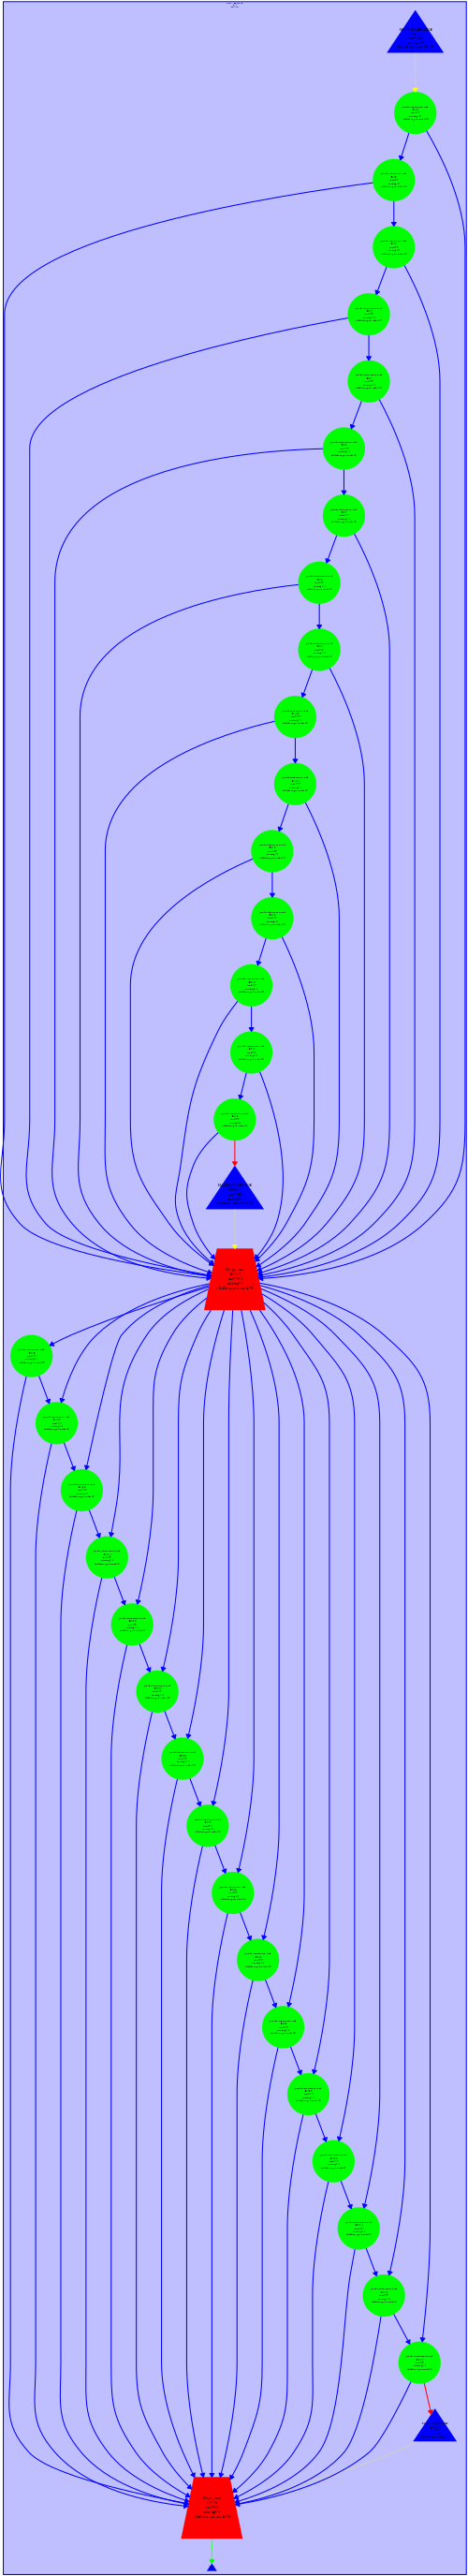
\includegraphics[scale=0.15]{./images/tareador-jacobi-2a}
\caption{\label{fig:TDGJacobi}}
\end{subfigure}
\begin{subfigure}{0.45\textwidth}
\centering
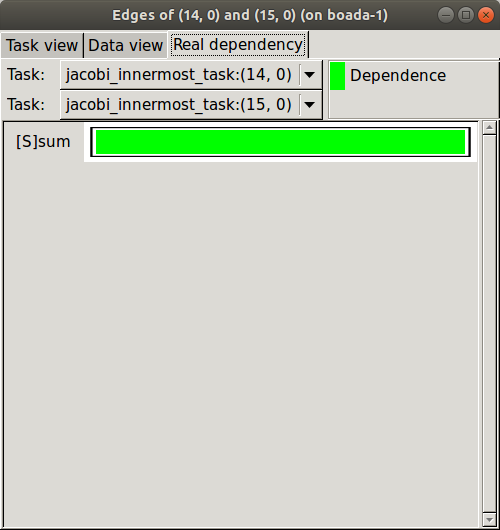
\includegraphics[scale=0.55,height=7cm]{./images/dependence-jacobi}
\caption{\label{fig:RealDependencyJacobi}}
\end{subfigure}
\caption{(a) Task decomposition graph for the Jacobi solver, (b) Real data dependences in the Jacobi solver.}
\end{figure}

Now, we know that the \textbf{sum} variable creates the dependences for the Jacobi solver. Novertheless, we have made use of some \textit{Tareador} calls that temporarily filter the analysis for the variable sum, causing the serialization and obtaining a new task graph (Figure \ref{fig:TDGJacobi-disable-sum}). The modified fragment of the code can be found in \textit{jacobi-tareador-disable-sum.c} file in the codes directory.

\begin{figure}[H]
\begin{lstlisting}
 double relax_jacobi (double *u, double *utmp, unsigned sizex,
 					  unsigned sizey)
 {
 	 ...
     for (int blockid = 0; blockid < howmany; ++blockid) {
       ...
       for (int i=max(1, i_start); i<= min(sizex-2, i_end); i++) {
         for (int j=1; j<= sizey-2; j++) {
			 tareador_start_task("jacobi_innermost_task");
			 ...
			 tareador_disable_object(&sum);
			 sum += diff * diff;
			 tareador_enable_object(&sum);
			 tareador_end_task("jacobi_innermost_task");
	 	 }
       }
     }

     ...
 }
\end{lstlisting}
\label{code:tareador-relax-jacobi-disable-sum}
\caption{Code for the task decomposition for relax\_jacobi function temporarily filtering the analysis of the sum variable.}
\end{figure}


\begin{figure}[H]
	\centering
	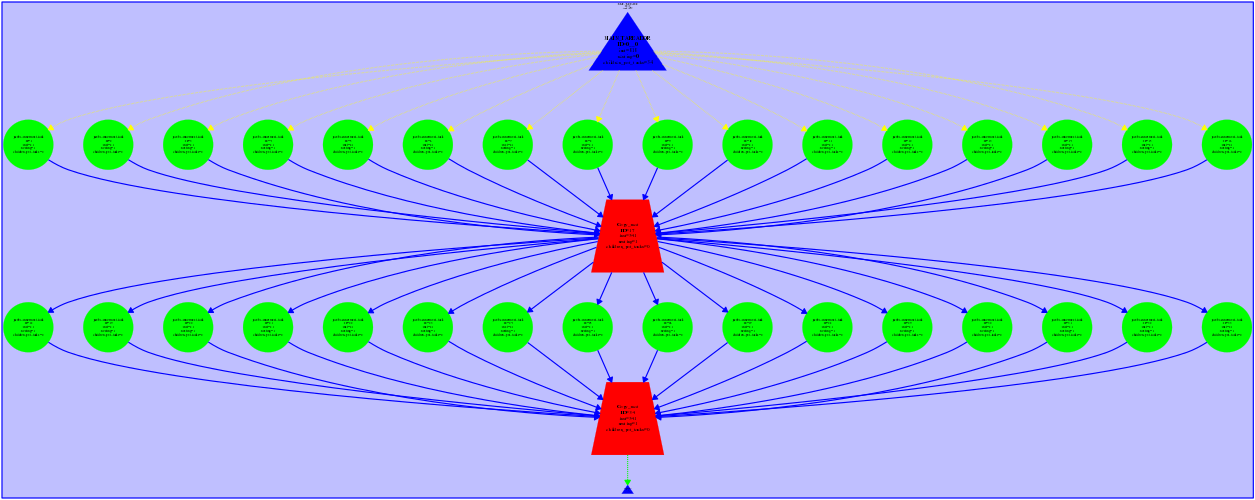
\includegraphics[scale=0.35]{./images/tareador-jacobi-2b}
	\label{fig:TDGJacobi-disable-sum}
	\caption{Task decomposition graph of the Jacobi solver temporarily filtering the analysis of the sum variable.}
\end{figure}

Now, we can see that there is any dependency between tasks of the most innerloop. Hence, we are increasing the parallelism. We think that the \textit{reduction(+:sum)} clause would be a good option to parallelise the code using \textit{OpenMP} directives.

\subsection{Gauss-Seidel Solver}

The Gauss-Seidel Solver does no longer use an auxiliar matrix. It writes in the position of the matrix where it reads the values. As in the previous solver, it takes the values of the element on its top and bottom and on its left and right, and does some arithmetic operations.

The modified code can be found in \textit{gauss-seidel-tareador.c} file in the codes directory.

\begin{figure}[H]
\begin{lstlisting}
 double relax_gauss (double *u, unsigned sizex, unsigned sizey)
 {
     double unew, diff, sum=0.0; 
 
     int howmany=1;
     for (int blockid = 0; blockid < howmany; ++blockid) {
       int i_start = lowerb(blockid, howmany, sizex);
       int i_end = upperb(blockid, howmany, sizex);
       for (int i=max(1, i_start); i<= min(sizex-2, i_end); i++) {
         for (int j=1; j<= sizey-2; j++) { 
			 tareador_start_task("gauss_seidel_innermost_task");
			 unew= 0.25 * ( u[ i*sizey	+ (j-1) ]+  // left
		 		   		    u[ i*sizey	+ (j+1) ]+  // right
				   		    u[ (i-1)*sizey	+ j     ]+  // top
				   		    u[ (i+1)*sizey	+ j     ]); // bottom
			 diff = unew - u[i*sizey+ j];
			
			 sum += diff * diff; 
			
		 	 u[i*sizey+j]=unew;
			 tareador_end_task("gauss_seidel_innermost_task");
         }
       }
     }

     return sum;
 }
\end{lstlisting}
\label{code:tareador-gauss-seidel}
\caption{Code for the task decomposition for relax\_gauss function.}
\end{figure}


The task decomposition graph is shown in Figure \ref{fig:TDGGaussSeidel}. We can observe that it has also some dependencies. Using the same procedure than in the previous section, we got the Real dependencies for this new solver (Figure \ref{fig:RealDependencyGaussSeidel}).

\begin{figure}[H]
\centering
\begin{subfigure}{0.45\textwidth}
\centering
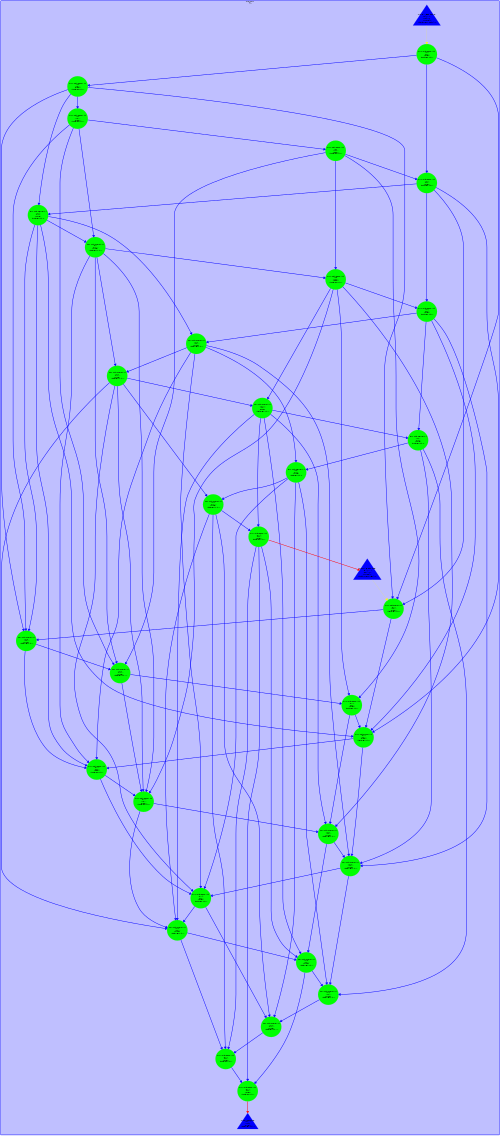
\includegraphics[scale=0.35]{./images/tareador-gauss-seidel-2a}
\caption{\label{fig:TDGGaussSeidel}}
\end{subfigure}
\begin{subfigure}{0.45\textwidth}
\centering
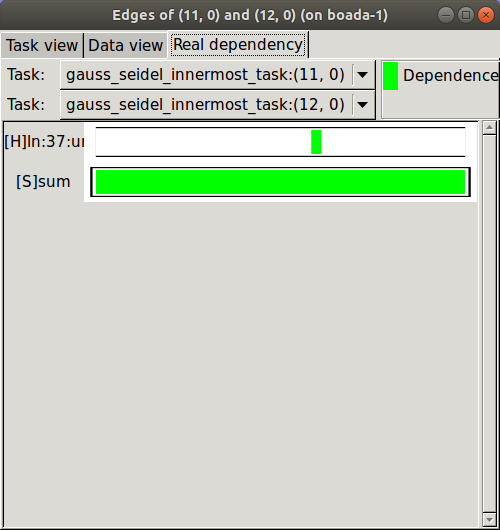
\includegraphics[scale=0.55,height=7cm]{./images/dependence-gauss-seidel}
\caption{\label{fig:RealDependencyGaussSeidel}}
\end{subfigure}
\caption{(a) Task decomposition graph for the Gauss-Seidel solver, (b) Real data dependences in the Gauss-Seidel solver.}
\end{figure}

We can see that this solver has two real dependencies: variable \textbf{sum} and some \textbf{positions of the matrix}. In this section, we will only show the TDG when disabling only the sum variable. However, the TDG of both variables disables can be found in the Annex section \ref{sec:TDGAllDisablesGaussSeidel}.

This new version of the code can be found in \textit{gauss-seidel-disable-sum.c}, in the codes directory.

\begin{figure}[H]
\begin{lstlisting}
 double relax_gauss (double *u, unsigned sizex, unsigned sizey)
 {
     ...
     for (int blockid = 0; blockid < howmany; ++blockid) {
       ...
       for (int i=max(1, i_start); i<= min(sizex-2, i_end); i++) {
         for (int j=1; j<= sizey-2; j++) {
			 tareador_start_task("gauss_seidel_innermost_task");
			 ...
			 tareador_disable_object(&sum);
			 sum += diff * diff; 
			 tareador_enable_object(&sum);
			 ...
			 tareador_end_task("gauss_seidel_innermost_task");
         }
       }
     }
     ...
 }
\end{lstlisting}
\label{code:tareador-relax-jacobi-disable-sum}
\caption{Code for the task decomposition for relax\_gauss function temporarily filtering only the analysis of the sum variable.}
\end{figure}


\begin{figure}[H]
	\centering
	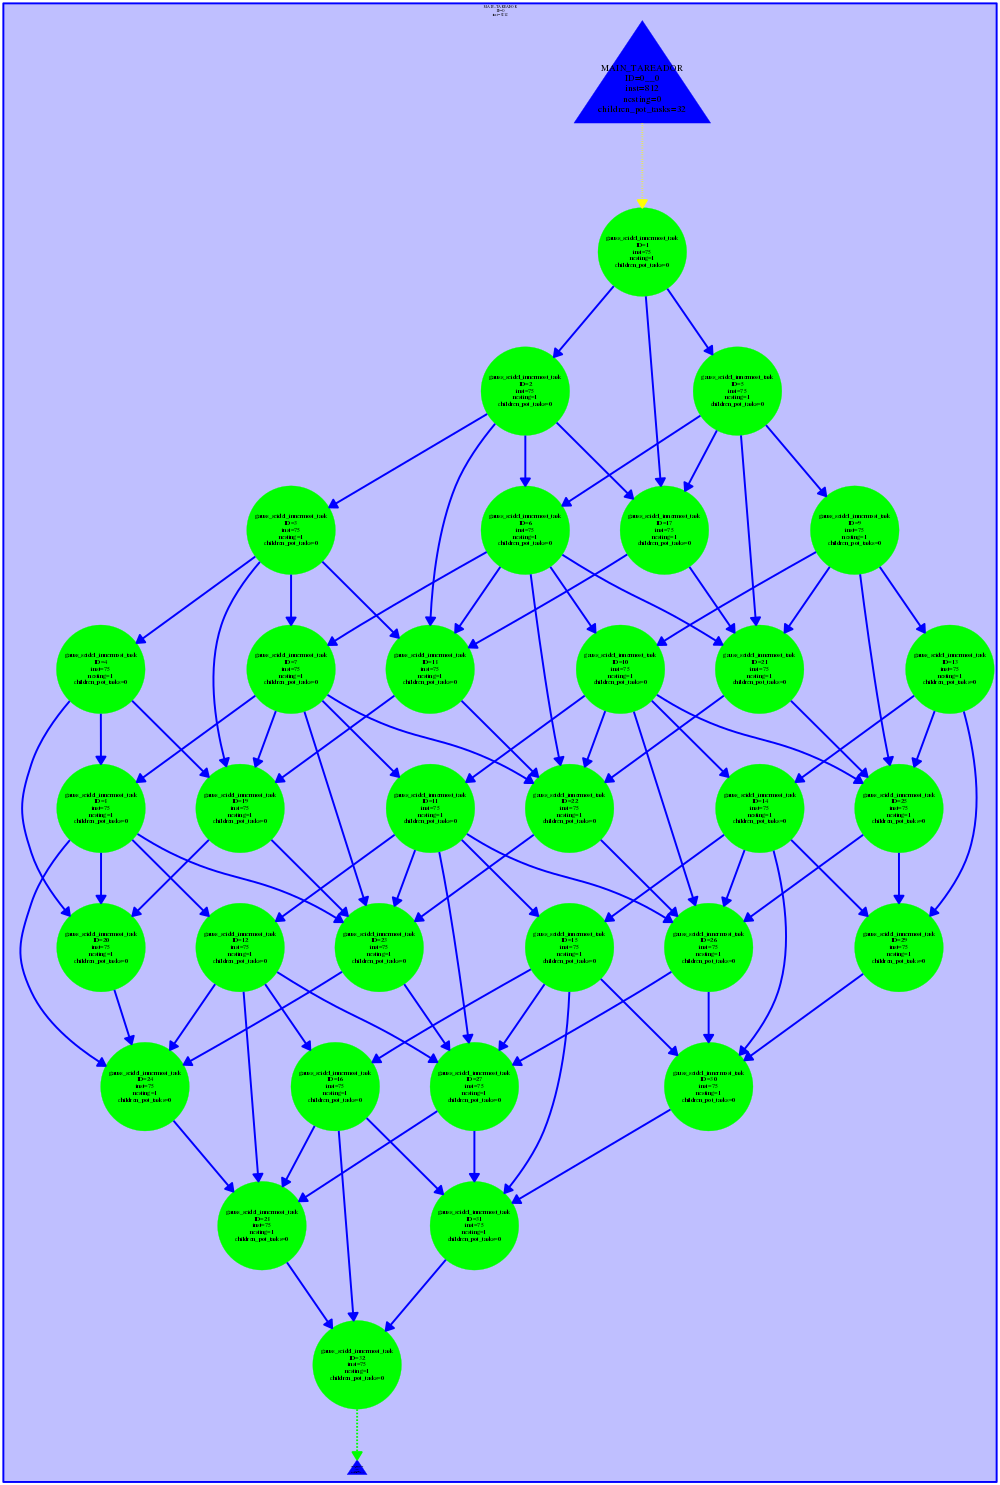
\includegraphics[scale=0.20]{./images/tareador-gauss-seidel-2b-sum}
	\label{fig:TDGGauss-Seidel-disable-sum}
	\caption{Task decomposition graph of the Gauss-Seidel solver temporarily filtering only the analysis of the sum variable.}
\end{figure}

Disabling temporarily the variable sum we see that we increase the parallelism. Again, we think that the \textit{reduction(+:sum)} clause would be good to porallelise the code using \textit{OpenMP} directives. Moreover, we can use the \textit{ordered} clause in order to avoid data races and respect the real dependencies we have seen (apply the doacross technique).


\section{Parallelization of \textit{Jacobi} with OpenMP \texttt{parallel}}
In this part of the laboratory, we had to understand the code that resolves the problem using the Jacobi algoithm, and afterwards parallelize it, in order to increase the speed of the execution.

\subsection{Understand the code}
The Jacobi algorithm has some functions created in order to facilitate the readability of the code. This functions are:

\begin{figure}[H]
\begin{lstlisting}
#define lowerb(id, p, n) ( id * (n/p) + (id < (n%p) ? id : n%p) )
#define numElem(id, p, n) ( (n/p) + (id < (n%p)) )
#define upperb(id, p, n) ( lowerb(id, p, n) + numElem(id, p, n) - 1 )
#define min(a, b) ( (a < b) ? a : b )
#define max(a, b) ( (a > b) ? a : b )
\end{lstlisting}
\caption{Given functions}
\end{figure}

The function lowerb and upperb returns the first and the last index of a vector partitons, when it is given an id (the partition number), p (the number of partitions) and n (the size of the vector).

The function numElem that returns the number of elements that are in a partition of a vector. Having the same entries as before.

And finally min and max functions that returns the minimum and maximum number between two respectively.

\begin{figure}[H]
	\centering
	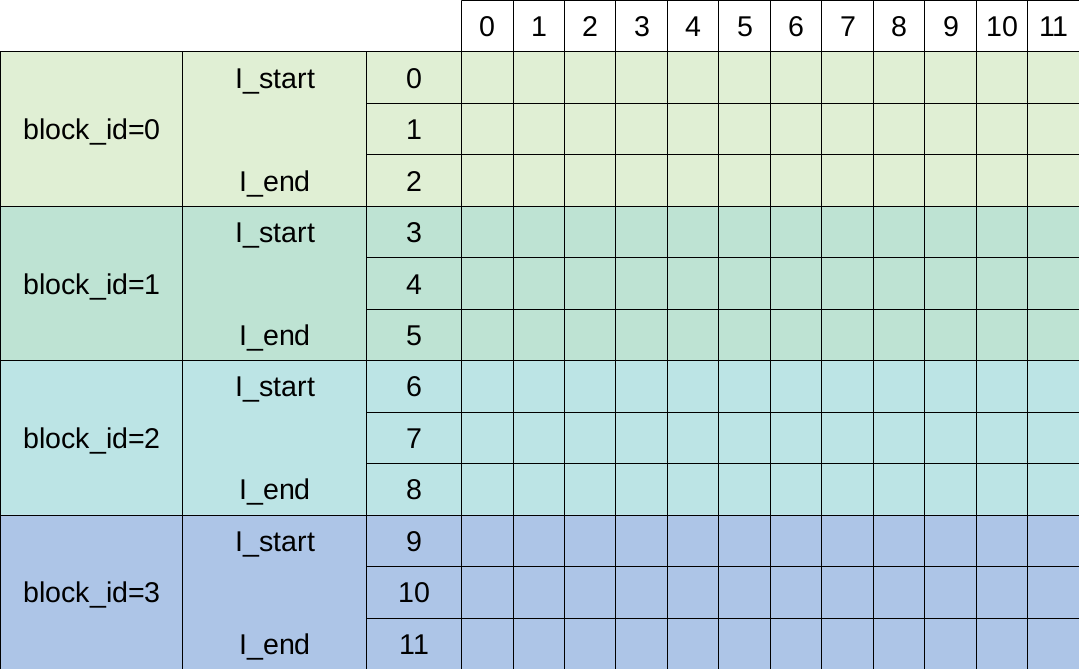
\includegraphics[scale=0.30]{./images/data_decomposition.png}
	\caption{Geometric data decomposition.}
	\label{fig:geometricdatadecomposition}
\end{figure}

In the geometric data decomposition we can see how the block\_id is distributed in a matrix (12 x 12). Assuming that in the code is using a vector to represent the matrix, the size of the vector would be 144.

\subsection{Parallelization of Jacobi}

In this part we had to parallelize the code considering that we want to create 4 blocks, without using \textit{\#pragma omp parallel for} clause in the code. To do that we have modified the relax\_jacobi function:

 \begin{figure}[H]
\begin{lstlisting}
double relax_jacobi (double *u, double *utmp, unsigned sizex, unsigned sizey)
{
	double diff, sum=0.0;

	int howmany = 4;
	#pragma omp parallel reduction(+: sum) private(diff)
	{
		int blockid = omp_get_thread_num();
		int i_start = lowerb(blockid, howmany, sizex);
		int i_end = upperb(blockid, howmany, sizex);
		for (int i=max(1, i_start); i<= min(sizex-2, i_end); i++) {
			for (int j=1; j<= sizey-2; j++) {
				 utmp[i*sizey+j]= 0.25 * ( u[ i*sizey + (j-1) ]+ // left
										   u[ i*sizey + (j+1) ]+ // right
							   			   u[ (i-1)*sizey + j ]+ // top
							               u[ (i+1)*sizey + j ]);// bottom
				 diff = utmp[i*sizey+j] - u[i*sizey + j];
				 sum += diff * diff; 
			}
		}
	}

    return sum;
}
\end{lstlisting}
\caption{Code for parallellization of relax\_jacobi function}
\end{figure}

As we can see we have divided the matrix in 4 parts. This will cause that, if we execute the code with 8 threads only the first 4 threads will have a valid blockid number, so the other 4 threads will recieve an out of bound \textit{i\_start} index. As we can see in the following image:

\begin{figure}[H]
	\centering
	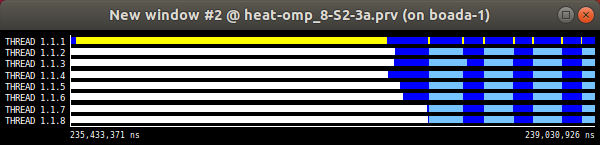
\includegraphics[scale=0.50]{./images/paraver-jacobi-s2-3a.png}
	\caption{Jacobi Schedule.}
\end{figure}

In order to solve that we modified a little bit more the \textit{relax\_jacobi} function.

 \begin{figure}[H]
\begin{lstlisting}
double relax_jacobi (double *u, double *utmp, unsigned sizex, unsigned sizey)
{
	double diff, sum=0.0;

	#pragma omp parallel reduction(+: sum) private(diff)
	{
		int howmany = omp_get_num_threads();
		....
	}

    return sum;
}
\end{lstlisting}
\caption{Improved code of relax\_jacobi function}
\end{figure}

Now we obtain a better parallelization in all the threads:

\begin{figure}[H]
	\centering
	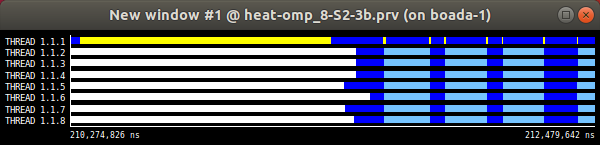
\includegraphics[scale=0.50]{./images/paraver-jacobi-s2-3b.png}
	\caption{Improved Jacobi Schedule.}
\end{figure}

But this wasn't enough parallel. In that moment we realised that the function \textit{copy\_mat} also has a big impact in the code. SO we decide to parallellize it.

 \begin{figure}[H]
\begin{lstlisting}
void copy_mat (double *u, double *v, unsigned sizex, unsigned sizey)
{
	#pragma omp parallel for collapse(2)
	for (int i=1; i<=sizex-2; i++)
		for (int j=1; j<=sizey-2; j++) 
			v[ i*sizey+j ] = u[ i*sizey+j ];
}
\end{lstlisting}
\caption{Code for parallellization of copy\_mat function}
\end{figure}

Now we obtained the best results regarding to parallelization. AS we can see in the following image:

\begin{figure}[H]
	\centering
	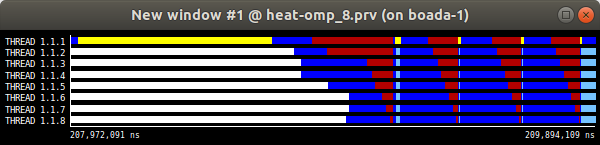
\includegraphics[scale=0.50]{./images/paraver-jacobi-s2-4.png}
	\caption{Improved Jacobi Schedule with copy\_mat parallellization.}
\end{figure}

Finally in order to test the scalability of our program. We executed the script \textit{submit-strong-omp.sh}, to obtain the following speed.up and scalability plots.

\begin{figure}[H]
	\centering
%	\includegraphics[scale=0.50]{}
	\caption{Jacobi scalability plots.}
\end{figure}

As we can see the performance increases together with the number of threads at first. But when we have a large number of threads the results shows a bit stagnation of this improvement.

\section{Parallelization of \textit{Gauss-Seidel} with OpenMP \texttt{ordered}}

In this section we have parallelized the Gauss-Seidel solver using \#pragma omp for and its \textbf{ordered} clause.

The important part with this solver was to decide how we would synchronize the parallel execution of the rows assigned to each processor in order to guarantee the dependences that we detected with \textit{Tareador}.

At first, we decided to divide the matrix as in figure \ref{fig:geometricdatadecomposition}. However, we realized that with that geometric data decomposition, the code would be executed exactly the same than in the sequential version because thread 1 would have had to wait until thread 0 terminated... Consequently, we had to think a new data decomposition.

The solution was to divide the matrix into blocks not only dividing the rows but the columns. Hence, when thread 0 finishes the first block, it continues excuting its new block whereas thread 1 can start executing its first block, and so on.

Then, we used again the \textbf{reduction(+:sum)} clause to improve the performance of the program without creating data races. Besides, we have also implemented the \textbf{doacross} technique using the \textbf{ordered(2)} clause, \textbf{\#pragma omp ordered depend(sink: ...)} and \textbf{\#pragma omp ordered depend(source)}. Each block can only be executed when blocks (i-1, j) and (i, j-1) terminate.

The code can be found in file \textit{gauss-seidel-reduction-doacross.c} in the codes directory.

\begin{figure}[H]
\begin{lstlisting}
 double relax_gauss (double *u, unsigned sizex, unsigned sizey) {
     double unew, diff, sum=0.0;
 
     #pragma omp parallel private(unew, diff) reduction(+: sum)
     {
	 int howmany = omp_get_num_threads();
	
	 #pragma omp for ordered(2) 
	 for (int blockid_i = 0; blockid_i < howmany; ++blockid_i) {
		 for (int blockid_j = 0; blockid_j < howmany; ++blockid_j) {
			 
			 int i_start = lowerb(blockid_i, howmany, sizex);
			 int i_end = upperb(blockid_i, howmany, sizex);
			 int j_start = lowerb(blockid_j, howmany, sizey);
			 int j_end = upperb(blockid_j, howmany, sizey);
			
			 #pragma omp ordered depend(sink: blockid_i-1,blockid_j)
			 for (int i=max(1, i_start); i<= min(sizex-2, i_end); i++) {
				 for (int j=max(1, j_start); j<= min(sizey-2, j_end); j++) {
					 unew= 0.25 * ( u[ i*sizey	+ (j-1) ]+  // left
								    u[ i*sizey	+ (j+1) ]+  // right
								    u[ (i-1)*sizey	+ j ]+  // top
								    u[ (i+1)*sizey	+ j ]); // bottom
					 diff = unew - u[i*sizey+ j];
					 sum += diff * diff; 
					 u[i*sizey+j]=unew;
				 }
			 }
			 #pragma omp ordered depend(source)
		 }
	 }
	 }
 
     return sum;
 }
\end{lstlisting}
\caption{Modified code of the function relax\_gauss.}
\end{figure}
 
Afterwards, we have used the \textit{Paraver} tool to see if the flow of the program matched our expectations. Due to the use of the \textbf{ordered} clause, we can see in Figure \ref{fig:trace-gauss-seidel-S4} that there is a lot of synchronization between threads. As we said before, thread 1 has to wait until thread 0 ends its first block, thread 2 has to wait until thread 1 terminated its first block... As a consequence, we see a kind of stairs at the beginning of each thread, in blue; and at the end of each thread execution, in red (the first thread will be the first to end, and so on).

\begin{figure}[H]
	\centering
	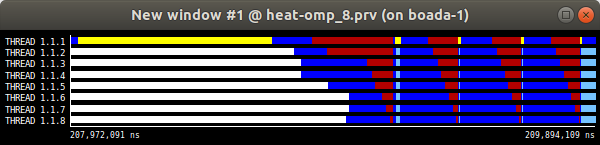
\includegraphics[scale=0.5]{./images/paraver-jacobi-s2-4}
	\caption{Traces obtained when executing the new version of relax\_gauss function.}
	\label{fig:trace-gauss-seidel-S4}
\end{figure}

Finally, we have analysed the scalability of our parallelization. We can see in Figures \ref{plot:exe-gauss} and \ref{plot:speed-gauss} that the results are worse than the plots in the Jacobi solver. The main reason is that this solver has more dependencies than Jacobi, so it has more synchronizations. Thus, it cannot have the same or better results.

\begin{figure}[H]
\centering
\hspace{-0.5cm}
\begin{minipage}{0.4\linewidth}
  \centering
  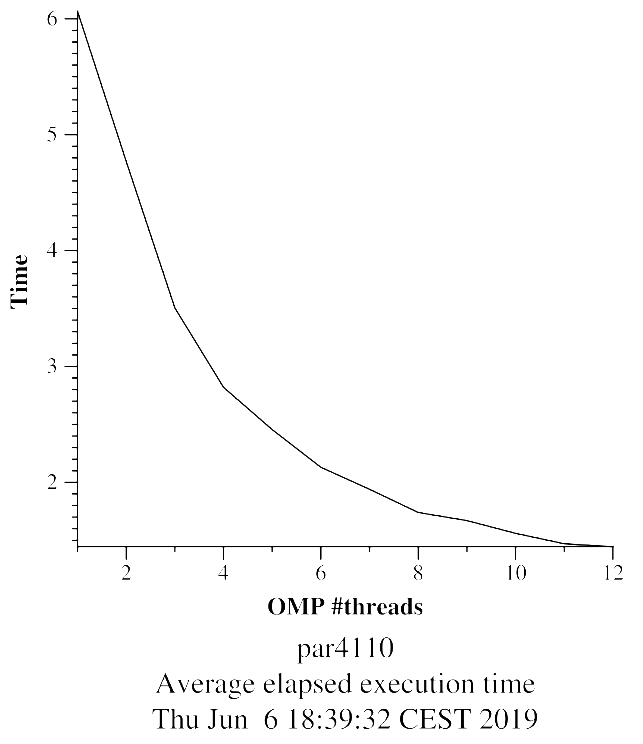
\includegraphics[scale=0.5]{./images/heat-omp-strong-gauss-execution-time}
  \caption{Execution time plot when varying the number of processors for the Gauss-Seidel solver.}
  \label{plot:exe-gauss}
\end{minipage}%
\hspace{0.5cm}
\begin{minipage}{0.4\linewidth}
  \centering
  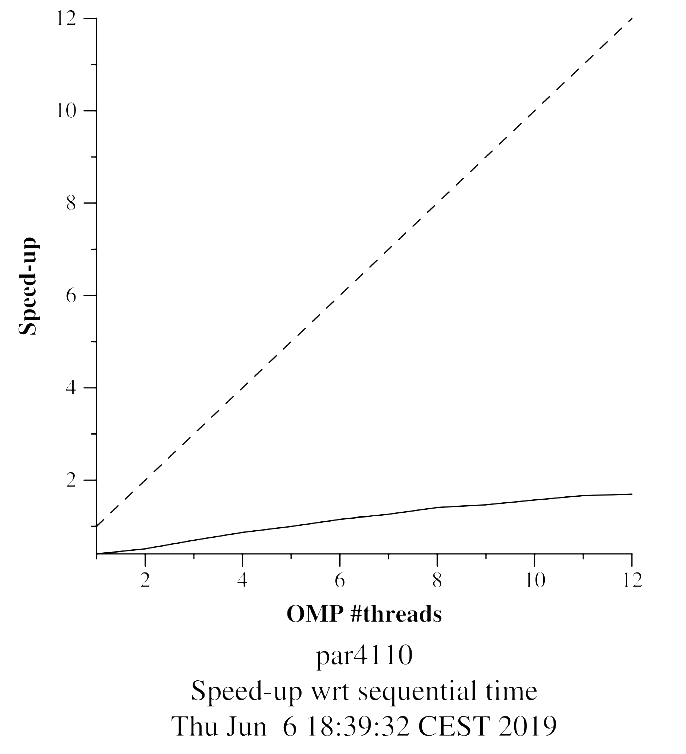
\includegraphics[scale=0.5]{./images/heat-omp-strong-gauss-speedup}
  \caption{Speedup plot when varying the number of processors for the Gauss-Seidel solver.}
    \label{plot:speed-gauss}
\end{minipage}
\end{figure}

\textbf{\large{\large{Encara FALTA mirar a baix.}}}

\newpage

How can you control in your code the trade-off between computation and synchronization? Is there
an optimum value for the ratio between computation and synchronization? For the execution with
8 threads, explore possible ratios and plot how the execution time varies.

Analyse the speed–up (strong scalability)
plot that has been obtained for the different numbers of processors, reasoning about the performance
that is observed and including captures of Paraver windows to justify your explanations. 






Finally explain
how did you obtain the optimum value for the ratio computation/synchronization in the parallelization
of this solver for 8 threads.





\section{Annex}
\subsection{Task dependency graph when also disabling temporarily some positions of the matrix}

In this section we will see the TDG created when disabling all the variables that create some kind of dependency in the Gauss-Seidel solver. The code can be found in \textit{gauss-seidel-disable-sum-and-matrix-positions.c}, inside the codes folder.

\begin{figure}[H]
\begin{lstlisting}
 double relax_gauss (double *u, unsigned sizex, unsigned sizey)
 {
     ...
     for (int blockid = 0; blockid < howmany; ++blockid) {
       ...
       for (int i=max(1, i_start); i<= min(sizex-2, i_end); i++) {
         for (int j=1; j<= sizey-2; j++) {
			 tareador_start_task("gauss_seidel_innermost_task");
 				
			 tareador_disable_object(&u[ i*sizey	+ (j-1) ]); // left
			 tareador_disable_object(&u[ (i-1)*sizey	+ j     ]); //top
			 unew= 0.25 * ( u[ i*sizey	+ (j-1) ]+  // left
 				   			u[ i*sizey	+ (j+1) ]+  // right
				    		u[ (i-1)*sizey	+ j     ]+  // top
				    		u[ (i+1)*sizey	+ j     ]); // bottom
			 diff = unew - u[i*sizey+ j];
			 tareador_enable_object(&u[ i*sizey	+ (j-1) ]);
			 tareador_enable_object(&u[ (i-1)*sizey	+ j     ]);
 			
			 tareador_disable_object(&sum);
			 sum += diff * diff; 
			 tareador_enable_object(&sum);
 			
			 ...
			 tareador_end_task("gauss_seidel_innermost_task");
         }
       }
     }
	 ...
 }
\end{lstlisting}
\caption{Code for the task decomposition for relax\_gauss function temporarily filtering the analysis of the sum variable and some positions of the matrix.}
\end{figure}

\begin{figure}[H]
	\centering
	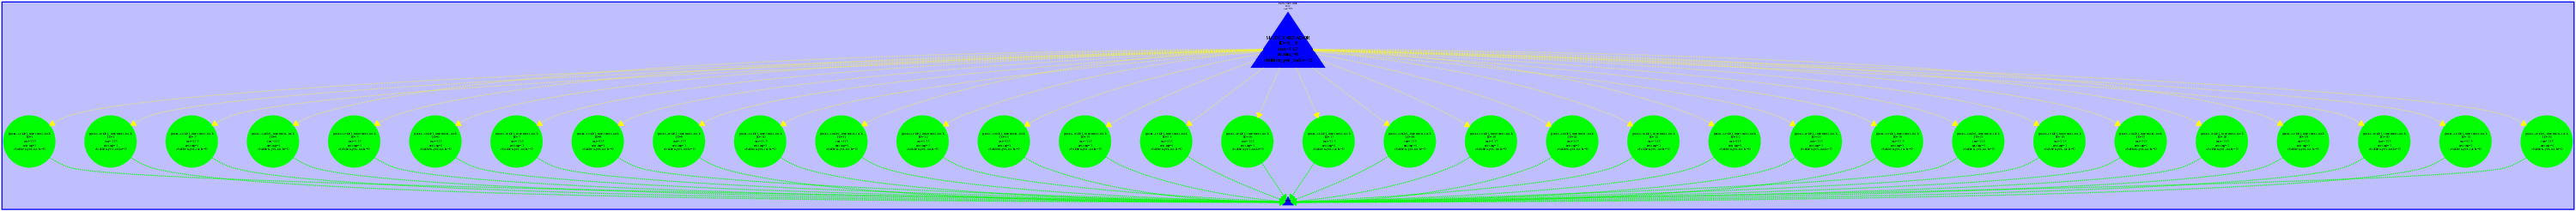
\includegraphics[scale=0.15]{./images/tareador-gauss-seidel-2b-sum-vector}
	\caption{Task decomposition graph of the Gauss-Seidel solver temporarily filtering the analysis of the sum variable and some positions of the matrix.}
\end{figure}

\label{sec:TDGAllDisablesGaussSeidel}



\end{document} 